\begin{frame}{Lifetimes in the self-organizing recurrent network}

  \vspace{0.55cm}
  
  % \large Define $D$ as the size of the STDP window for depression, divided by the size of the STDP for potentiation,

    \vspace{-0.4cm}

  \begin{figure}
    \centering
    \includegraphics<1>[width=0.925\textwidth]{%
      % figures/netlf1.png} %
      /home/fh/sci/lab/syn_lt/sorn_model/set_02/img/fpt_lfsn-long_green.png}
  \end{figure}

    \vspace{-0.2cm}

  \Large
  \begin{align*}
    D = \text{LTD--LTP balance}
  \end{align*}

  
\pnote{
  
  Does not depend on

  -- network size

  -- membrane noise levels

  -- exact synaptic scaling implementation
  
}
  
  
  
\end{frame}


\begin{frame}{Lifetimes modelled by a stochastic process}

  \vspace{0.55cm}

  \large Kesten process (\cite{Kesten1973, Statman2014})

  \begin{align*}
  X_{n+1} = a_n X_n + b_n
  \end{align*}

  as a model for synapse dynamics

  \vspace{0.3cm}

  \begin{figure}
    \centering
    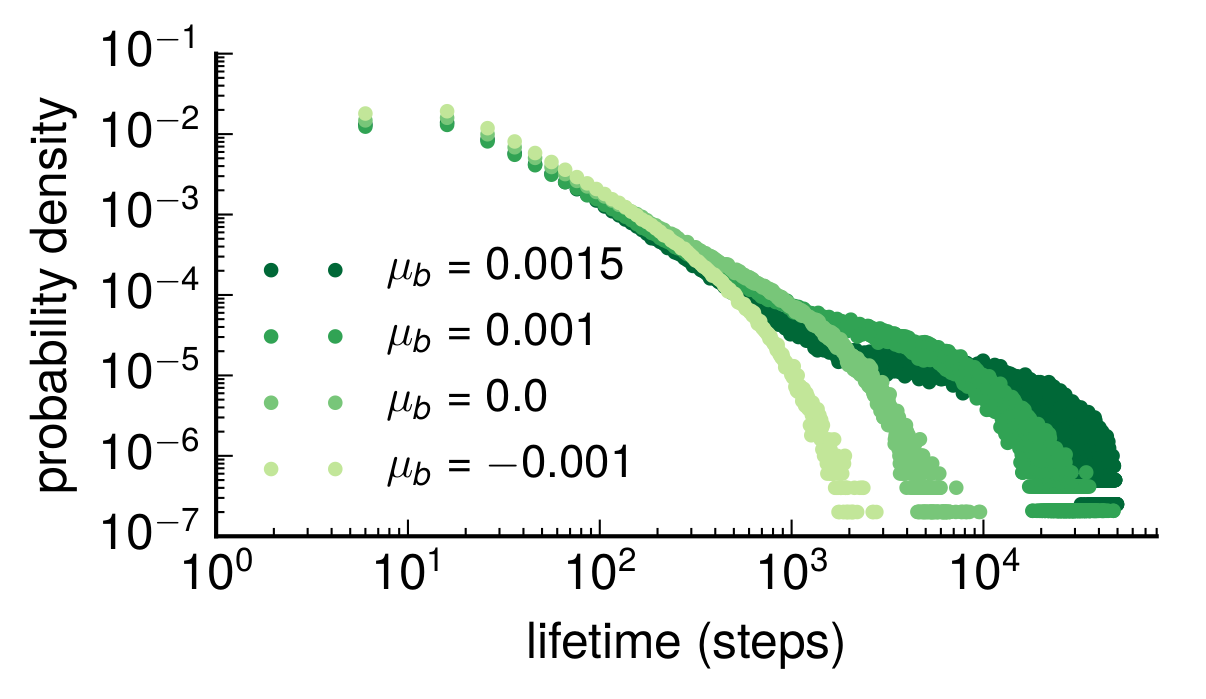
\includegraphics[width=0.85\textwidth]{%
      figures/lft1.png} %
  \end{figure}
  

  
  
\end{frame}

